%!TEX root = ../dissertation.tex

\graphicspath{{6-pilot/figures/}}

\newcommand\secondpilottitle{ Deep Generative Pitch and Timbre Modeling }
\chapter[Pilot Study 2: \newline \secondpilottitle]{~~~~~~~~~~~~~~~~~~~~~~~~~~~~~~~~~Pilot Study 2: \newline\vspace{-0.5em}\newline \secondpilottitle}
\label{ch:pilot2}

\TODO{this chapter is to be expanded}

\section{Generative Adversarial Network of Instrumental Sounds}


As seen in Chapter \ref{ch:deeplearning}, the recent surge of GAN variants have shown many promising results in computer vision.
To examine the potential applicability of a GAN model in music, a few attempts were made to train GANs that learns from musical sounds, in the form of raw audio waveforms and magnitude spectrograms.
A difference between audio and images is that audio has much more high-dimensional data than the typical images used in deep learning.
Time domain signals have tens of thousands of numbers for a second of audio, and a typical resolution of a magnitude spectrogram ranges from 512 to 1024 vertical pixels where many image datasets for deep learning is under 96 pixels.
Despite this difficulty, a careful design using mode regularized generative adversarial network (MRGAN) \cite{che2016mrgan} could achieve a stable convergence of 512-by-64 images of magnitude spectrograms, as shown in Figure \ref{fig:gan}.

\begin{figure}
	\centering
	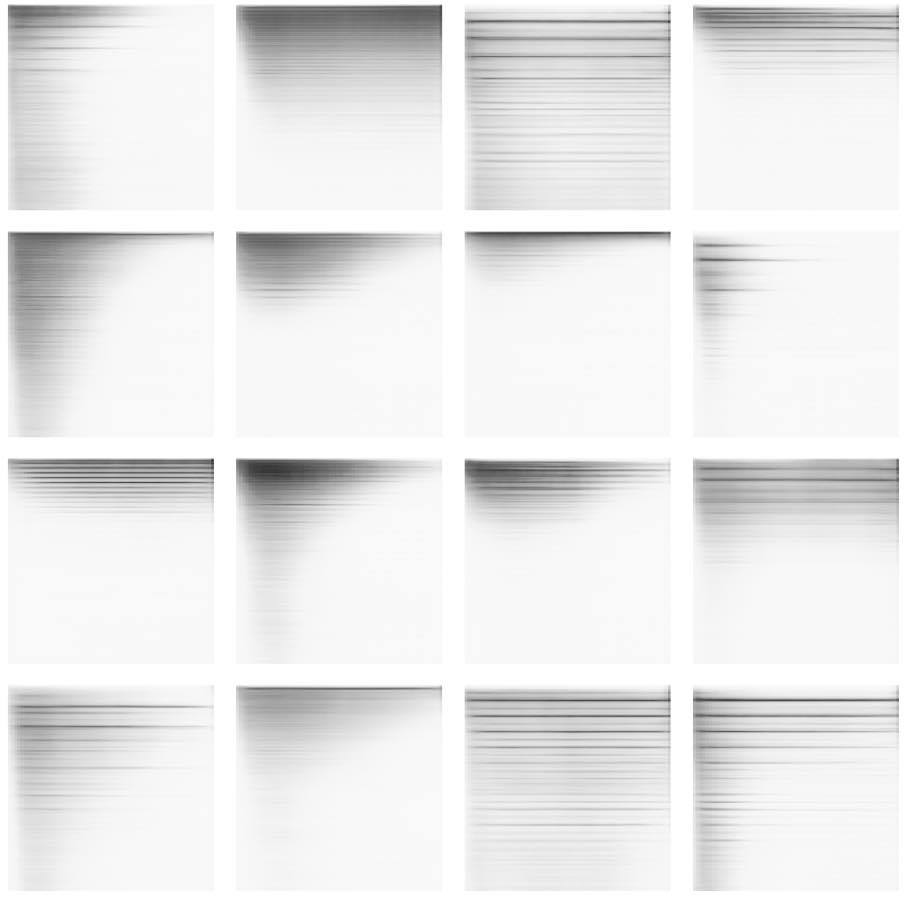
\includegraphics[width=0.9\textwidth]{gan.jpg}
	\caption{Spectrogram images generated by mode regularized generative adversarial network (MRGAN) %\cite{che2016mrgan} trained on instrumental sounds of Vienna symphonic library
	}\label{fig:gan}
\end{figure}

Future work in this project includes quantifying how the manifold learned by the GAN is informative in predicting various qualities of the sound, by combining the model with other GAN variants like InfoGAN \cite{chen2016infogan} or ACGAN \cite{odena2016acgan}.
Using NSynth dataset will also help in getting more insights of GAN's ability, since it is more organized and comes with more consistent annotations than Vienna Symphonic Library.

